\chapter{Grundlagen}
\label{sec:grundlagen}


\section{Software-Qualität}
\label{sec:softwarequalität}

Nahezu jeder Programmierer ist schon einmal mit dem Begriff der Software-Qualität in Berührung gekommen. Diesen Qualitätsbegriff jedoch genau zu fassen erweist sich als schwierig.
Die DIN-ISO-Norm 9126 definiert den Begriff Software-Qualität wie folgt:
\\
\glqq Software-Qualität ist die Gesamtheit der Merkmale und Merkmalswerte eines Software-Produkts, die sich auf dessen Eignung beziehen, festgelegte Erforderniss zu erfüllen.\grqq \cite{iso/iec_iso/iec_2001}
\\
Aus dieser Definition wird deutlich, dass es sich bei dem Begriff der Software-Qualität eine multikausale Größe handelt. Das bedeutet, dass zur Bestimmung der Qualität einer Software nicht ein einzelnes Kriterium existiert. Vielmehr verbergen sich hinter dem Begriff eine ganze Reihe verschiedener Kriterien die je nach den gestellten Anforderungen in ihrer Relevanz variieren.\cite[vgl. Seite 6 ff.]{hoffmann_software-qualitat_2013}
Sammlungen solcher Kriterien werden in sogenannten Qualitätsmodellen zusammengefasst. Die DIN-ISO-Norm 9126 bietet selbst ein solches Qualitätsmodell und definiert damit eine Reihe von wesentlichen Merkmalen, die für die Beurteilung der Software-Qualität eine Rolle spielen. Diese Merkmale sind in der Abbildung \ref{fig:qualitaetsmerkmaleVonSoftwaresystemen} zusammengefasst.
\begin{figure}[htb]
  \centering  
  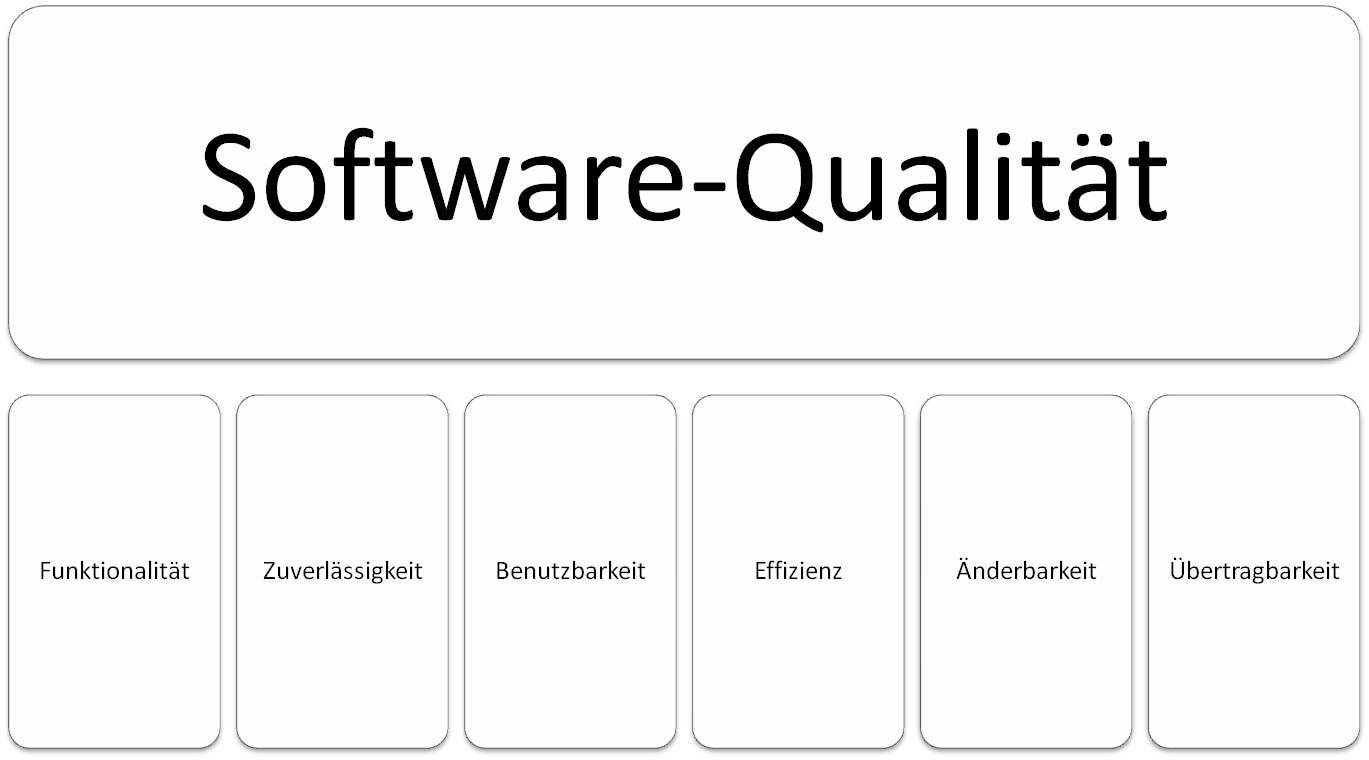
\includegraphics[scale=0.6]{img/softwarequalitaet9126.png}\\
  \footnotesize\sffamily\textbf{Quelle:} \cite{iso/iec_iso/iec_2001}
  \caption{Qualitätsmerkmale von Softwaresystemen (ISO 9126)}
  \label{fig:qualitaetsmerkmaleVonSoftwaresystemen}
\end{figure}
Eine nähere Definition der einzelnen Begriffe des Qualitätsmodells kann beispielsweise dem Buch Software-Qualität von Dirk W. Hoffmann entnommen werden. \cite[Seite 7 ff.]{hoffmann_software-qualitat_2013}
Um die Qualität einer Software zu Steigern bietet die moderne Software-Qualitätssicherung eine Vielzahl von Methoden und Techniken.
Ein Teil der Methoden geht dabei davon
aus, dass ein qualitativ hochwertiger Prozess der Produkterstellung die Entstehung von qualitativ hochwertigen Produkten begünstigt. Das Augenmerk wird hierbei also auf die Prozessqualität gelegt. Diese Methoden fallen in den Bereich der Prozessqualität.
Die klassischen Vorgehensmodelle der Softwarentwicklung
werden z.B. hier eingeordnet. Einen weiteren Bereich bilden die Methoden die zur Verbesserung der  Produktqualität dienen. Bei diesen Methoden wird das Softwareprodukt direkt bezüglich der Qualitätsmerkmale überprüft. Dieser Bereich unterteilt sich in die konstruktiven und analytischen Qualitätssicherung. Unter konstruktiver Qualitätssicherung versteht man den Einsatz von z.B. Methoden, Werkzeugen oder Standards die
dafür sorgen, dass ein Produkt bestimmte Forderungen erfüllt. 
Unter analytische Qualitätssicherung versteht man den Einsatz von analysierenden bzw. prüfenden Verfahren, die Aussagen
über die Qualität eines Produkts machen.
In diesem Bereich der Qualitätssicherung befindet sich beispielsweise der klassische Software-Test.\cite[vgl. Seite 19 ff.]{hoffmann_software-qualitat_2013} Eine Übersicht über das gesamte Gebiet der SoftwareQualitätssicherung, wie es sich uns gegenwärtig darstellt, ist in Abbildung \ref{fig:softwareQualitätssicherung} dargestellt. 
\begin{figure}[htb]
  \centering  
  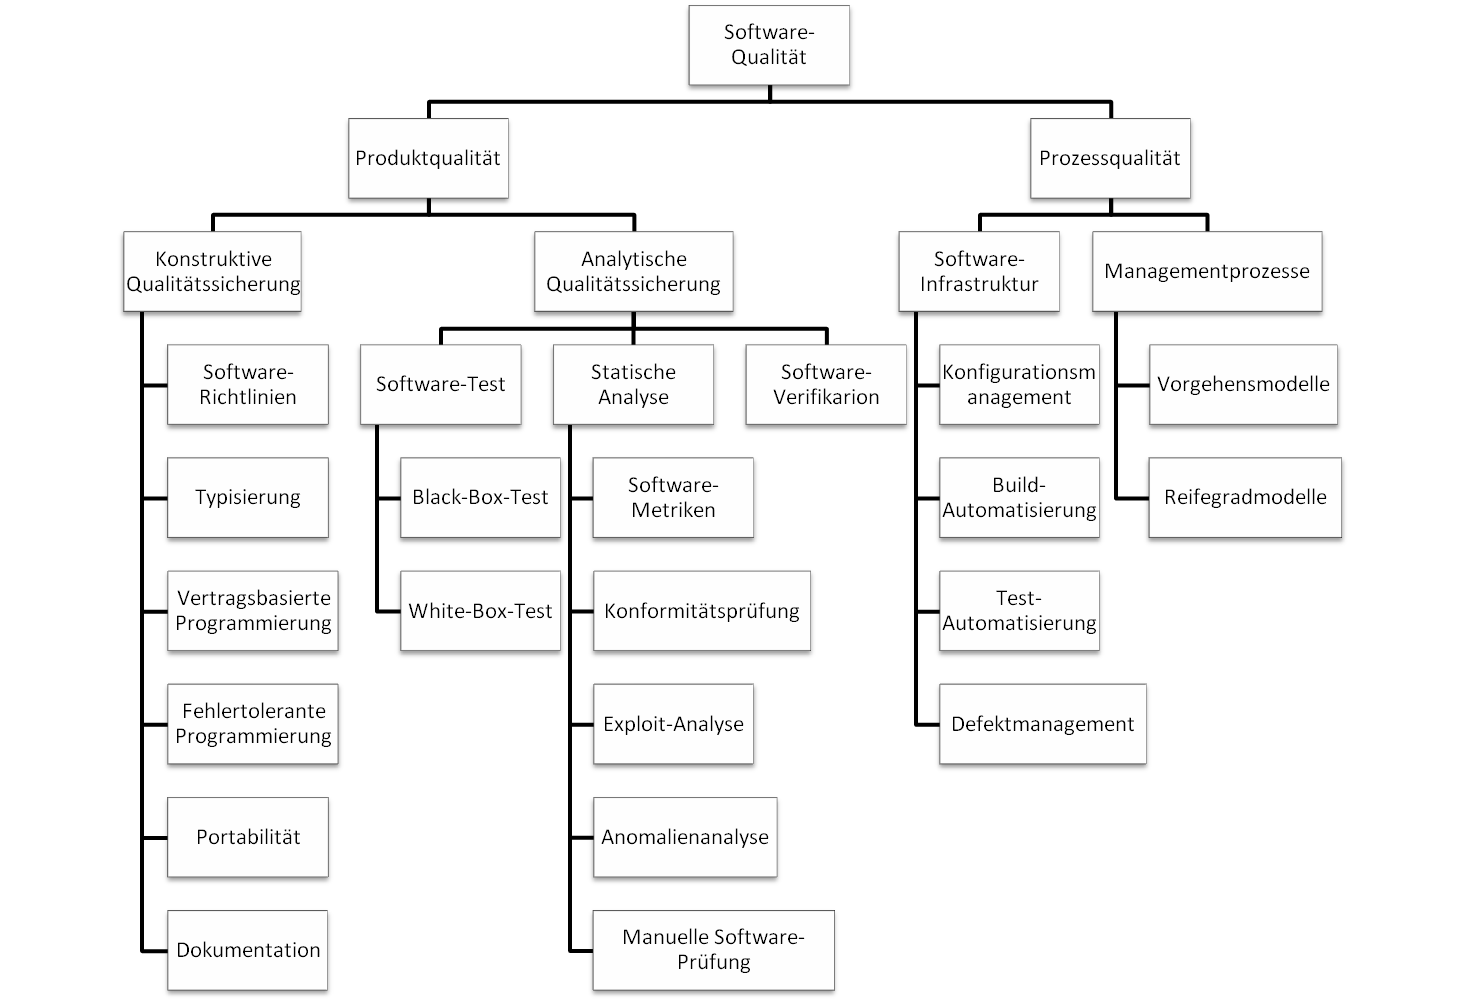
\includegraphics[scale=0.7]{img/softwarequalitaet.png}\\
  \footnotesize\sffamily\textbf{Quelle:} \cite[vgl. Seite 20]{hoffmann_software-qualitat_2013}
  \caption{Übersicht über das Gebiet der Software-Qualitätssicherung}
  \label{fig:softwareQualitätssicherung}
\end{figure}



\section{Softwaretest}
\label{sec:softwaretest}
In kapitel.. hben wir geseehn, dass der softwertest in .. angesiedelt ist.

\section{Testautomatisierung}
\label{sec:testautoGrundlagen}


\section{Testprozess}
\label{sec:testprozess}



\subsection{Testplanung und Steuerung}
\label{subsec:testplanung_und_steuerung}


\subsection{Testanalyse und Testdesign}
\label{subsec:testanalyse_und_design}


\subsection{Testrealisierung und Testdurchführung}
\label{subsec:testrealisierung_und_durchführung}

\subsection{Testauswertung und Bericht}
\label{subsec:testauswertung_und_bericht}


\subsection{Abschluss der Testaktivitäten}
\label{subsec:abschluss_der_testaktivitäten}



\section{Softwarelebenszyklus}
\label{sec:softwarelebenszyklus}



\subsection{V-Modell}
\label{subsec:vmodell}
\subsection{Agil}
\label{subsec:agil}

